% =====================================================================
%  Capítulo 1 — Introducción
% =====================================================================
\chapter{Introducción}
\citacap{En los campos de la observación, la suerte favorece únicamente a la mente preparada.}{Louis Pasteur}

El \textbf{objetivo} de este manual es lograr la mentalización necesaria para hacer frente a una situación en la que somos objeto de una agresión, potenciando nuestras habilidades y capacidades de defensa. Esta edición revisada está orientada específicamente a la mujer, e incorpora los avances de los últimos años en tres frentes: la evidencia científica sobre la eficacia de la autodefensa femenina, la actualización del marco legal español y las nuevas herramientas tecnológicas (aplicaciones móviles de seguridad ciudadana).

\textbf{La defensa personal NO es un arte marcial.} La mayoría de las artes marciales se han transformado en disciplinas competitivas donde se entrenan técnicas deportivas ---con sus normas--- en un ámbito protegido (monitores y árbitros). En la defensa personal el ambiente no es protegido y el objetivo es único: interrumpir la agresión y escapar.

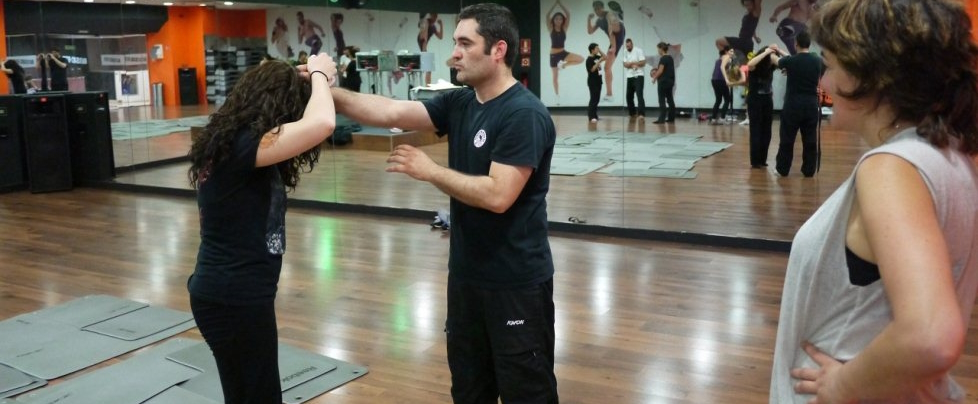
\includegraphics[width=\linewidth]{figures/02.jpg}

Dada la simplicidad de las técnicas de defensa personal, no se requieren años de práctica para poder aplicarlas. Pero debe quedar claro que la \enquote{magia} de las artes marciales consiste precisamente en la repetición de las técnicas infinidad de veces para que se interioricen y se expresen espontáneamente cuando sean necesarias. Esto es también aplicable a la defensa personal: las técnicas deberán practicarse y repasarse mentalmente hasta que su ejecución sea automática. Nadie puede esperar adquirir esta capacidad únicamente leyendo un manual.

La buena noticia es que hoy sabemos, con datos, que esto funciona. Un ensayo controlado aleatorizado publicado en el \emph{New England Journal of Medicine} \citep{senn2015} demostró que un programa de resistencia y autodefensa de 12 horas redujo en un 46\,\% el riesgo de violación consumada entre universitarias durante el año siguiente. Otros estudios \citep{hollander2014, sarnquist2014} confirman que el entrenamiento en autodefensa con enfoque de empoderamiento reduce la victimización y aumenta la confianza, sin trasladar la responsabilidad del delito a la víctima: la responsabilidad de una agresión es siempre, y únicamente, del agresor.

Se debe adquirir paulatinamente un pensamiento previsor de actitudes defensivas, aplicables ante ataques en los lugares que frecuentamos (imaginarnos qué haríamos si en la próxima esquina apareciese alguien que nos amenaza).

\textbf{En resumen:} no se trata solo de dominar unas técnicas de defensa, sino de prepararse mentalmente (atención y confianza) para una situación en la que debamos utilizarlas.

\begin{aviso}
\textbf{Aviso importante.} Este manual tiene fines educativos y no sustituye la formación presencial con instructores cualificados, ni el asesoramiento legal, médico o psicológico profesional. Si estás sufriendo violencia, en España puedes llamar al \recurso{016} (gratuito, 24\,h, no aparece en la factura) o al \recurso{112} en caso de emergencia.
\end{aviso}
